\section{Thiết kế}
    \subsection{Kiến trúc Hệ thống}
        \subsubsection{Sơ đồ khối Hệ thống}
            \begin{figure}[h]
                \centering
                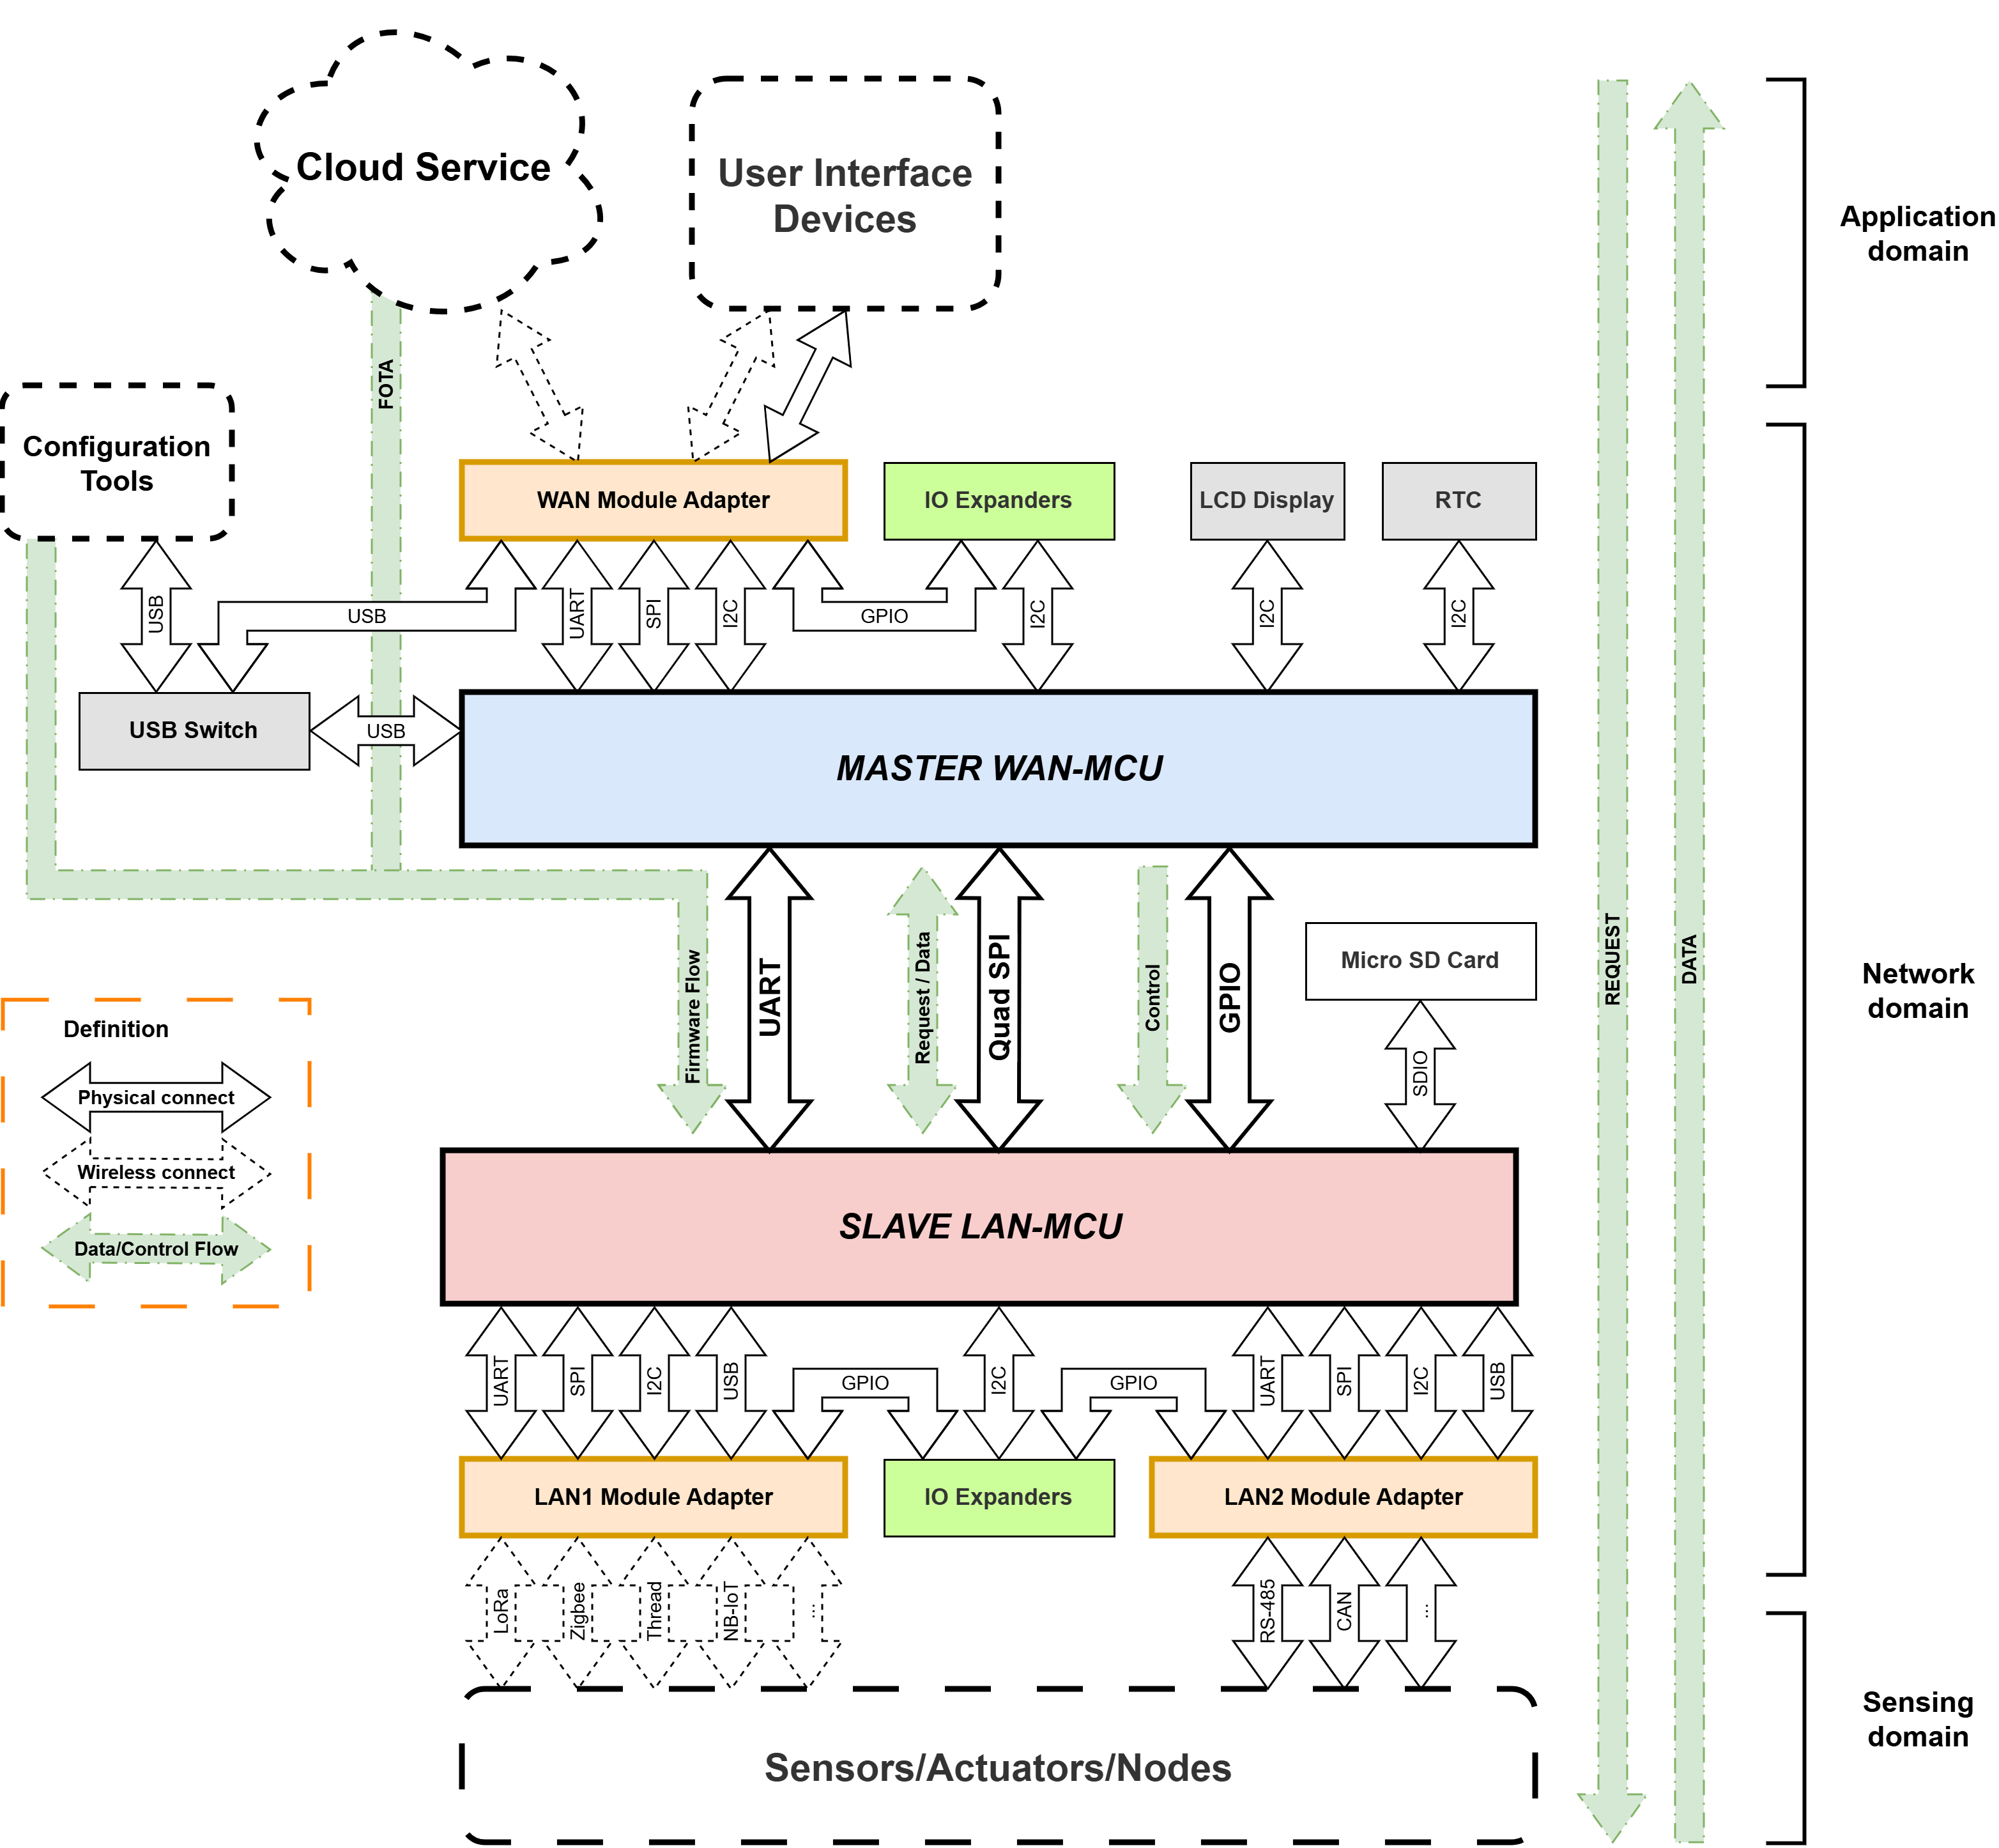
\includegraphics[width=0.8\textwidth]{figures/Protype_SystemBlockDiagram_Draft-System Block Diagram.drawio.png}
                \caption{Sơ đồ khối Hệ thống}
            \end{figure}
            
        \subsubsection{Mô tả thành phần hệ thống}
            Hệ thống được thiết kế theo mô hình Dual-MCU Master-Slave, chia thành 3 miền chức năng chính: Application Domain (Ứng dụng), Network Domain (Mạng lưới xử lý), và Sensing Domain (Cảm biến).
            \paragraph{Baseboard:}\par
                Là board chính của hệ thống, chịu trách nhiệm cung cấp nguồn điện ổn định, giao tiếp giữa các thành phần, kết nối với Module Adapter, và chứa các vi điều khiển chính.

            \paragraph{Khối Xử lý trung tâm:}\par
                Hệ thống sử dụng kiến trúc xử lý song song với hai vi điều khiển chuyên biệt nhằm tối ưu hóa hiệu năng và tài nguyên phần cứng:
                \begin{itemize}
                    \item \textbf{MASTER WAN-MCU}
                    \begin{itemize}
                        \item Vai trò: Là vi điều khiển chính, chịu trách nhiệm xử lý các tác vụ thuộc Lớp ứng dụng (Application Layer) và điều phối hoạt động cả hệ thống.
                        \item Chức năng: Xử lý các tác vụ Lớp ứng dụng thông qua WAN Module Adapter, quản lý giao diện người dùng và kết nối đám mây, điều phối luồng dữ liệu chính, và điều phối hoạt động của SLAVE LAN-MCU. MASTER WAN-MCU chịu trách nhiệm cập nhật firmware từ thiết bị cấu hình (Configuration Tools) và từ đám mây (FOTA) cho cả hệ thống.
                    \end{itemize}
                    \item \textbf{SLAVE LAN-MCU}
                    \begin{itemize}
                        \item Vai trò: Chịu trách nhiệm tương tác trực tiếp với lớp Cảm biến (Sensing Domain), quản lý các kết nối mạng nội bộ thông qua LAN Module Adapter, và lưu trữ dữ liệu.
                        \item Chức năng: Quản lý các giao thức truyền thông nội bộ và mạng cảm biến, thu thập dữ liệu thô, thực hiện tiền xử lý và lưu trữ cục bộ (Micro SD Card) trước khi gửi lên MASTER WAN-MCU.
                    \end{itemize}
                \end{itemize}

            \paragraph{Giao tiếp giữa hai Vi xử lý:}\par
                Để đảm bảo đồng bộ dữ liệu giữa MASTER WAN-MCU và SLAVE LAN-MCU, hệ thống sử dụng ba đường giao tiếp riêng biệt:
                \begin{itemize}
                    \item \textbf{Quad SPI (Request/Data)}: Kênh truyền dữ liệu tốc độ cao, dùng để Slave gửi dữ liệu cảm biến lên Master và Master gửi yêu cầu xuống Slave.
                    \item \textbf{UART (Firmware Flow)}: Kênh chuyên biệt dùng để nạp firmware cho SLAVE LAN-MCU thông qua MASTER WAN-MCU
                    \item \textbf{GPIO (Control)}: Các đường tín hiệu điều khiển (Boot, Reset, Interrupt) để đảm bảo đồng bộ trạng thái hoạt động.
                \end{itemize}

            \paragraph{Khối Module Adapter}\par
                Đây là thành phần cho phép tháo lắp và thay thế linh hoạt các module, được chuẩn hóa kết nối với Baseboard gồm các giao thức: UART, SPI, I2C, USB, và các GPIO.
                \begin{itemize}
                    \item \textbf{WAN Module Adapter}
                    \begin{itemize}
                        \item Kết nối với MASTER WAN-MCU.
                        \item Hỗ trợ các module giao tiếp với Cloud hoặc thiết bị người dùng (User Interface Devices).
                    \end{itemize}
                    \item \textbf{LAN1 Module Adapter}
                    \begin{itemize}
                        \item Kết nối với SLAVE LAN-MCU.
                        \item Hỗ trợ kết nối các module kết nối không dây như LoRa, Zigbee, BLE, Thread, NB-IoT, \dots
                    \end{itemize}
                    \item \textbf{LAN2 Module Adapter}
                    \begin{itemize}
                        \item Kết nối với SLAVE LAN-MCU.
                        \item Hỗ trợ kết nối các module kết nối có dây như RS-485, CAN, \dots
                    \end{itemize}
                \end{itemize}

            \paragraph{Thiết bị giao diện người dùng (User Interface Devices):}\par
                Các thiết bị đầu cuối giúp người quản trị tương tác với hệ thống thông qua các giao thức mạng không dây như Wi-Fi hay có dây như Ethernet.
            \paragraph{Cloud Service:}\par
                Nền tảng đám mây cung cấp dịch vụ lưu trữ, phân tích dữ liệu và quản lý tập trung cho hệ thống IoT.
            \paragraph{Configuration Tools:}\par
                Một chương trình máy tính để cấu hình cho gateway thực hiện những chức năng cho các module được kết nối.
            \paragraph{Luồng dữ liệu:}\par
                \begin{itemize}
                    \item \textbf{Firmware/FOTA Flow:} Firmware được nạp vào thiết bị thông qua Configuration Tools bằng kênh USB, hoặc từ đám mây (FOTA) qua MASTER WAN-MCU, sau đó được chuyển tiếp đến SLAVE LAN-MCU qua kênh UART chuyên biệt.
                    \item \textbf{Request/Data Flow:} Request được gửi từ Miền Ứng dụng (Application Domain) qua MASTER WAN-MCU đến SLAVE LAN-MCU để lấy dữ liệu cảm biến. Dữ liệu cảm biến sau khi được thu thập và tiền xử lý tại SLAVE LAN-MCU, hoặc đang được lưu trữ sẽ được gửi ngược lại qua MASTER WAN-MCU lên Cloud Service. Các request và dự liệu này được truyền qua kênh Quad SPI tốc độ cao kết nối giữa hai MCU.
                    \item \textbf{Control Flow:} Luồng tín điều khiển từ MASTER WAN-MCU để điều khiển trạng thái hoạt động của SLAVE LAN-MCU, và điều khiển hệ thống nguồn điện cho gateway thông qua các đường GPIO.
                \end{itemize}

        \subsubsection{Thiết kế Module hóa}
            \paragraph{Nguyên lý:}\par
                Thiết kế module hóa cho phép người dùng dễ dàng thay thế, nâng cấp hoặc mở rộng các chức năng của gateway mà không cần thay đổi toàn bộ hệ thống. Mỗi module được thiết kế theo chuẩn kết nối chung, giúp đảm bảo tính tương thích và linh hoạt trong việc lựa chọn các module phù hợp với nhu cầu sử dụng cụ thể.
            \paragraph{Thiết kế:}\par
                Đối với các module có sẵn trên thị trường, các module này thông thường sẽ không theo một tiêu chuẩn cụ thể kể cả các module dạng Mini PCIe hay M.2, do đó việc thiết kế các Module Adapter đóng vai trò quan trọng trong việc chuẩn hóa kết nối giữa các module và Baseboard.
            \paragraph{Chuẩn hóa giao diện:}\par
                Mỗi Module Adapter được thiết kế với các giao diện chuẩn bao gồm UART, SPI, I2C, USB, và GPIO được định nghĩa sơ đồ chân:
                \begin{longtable}{|l|l|p{5cm}|l|}
                    \hline
                    \textbf{Group} & \textbf{Pin Name} & \textbf{Pin Number} & \textbf{Description} \\\hline
                    \endfirsthead
                    \hline
                    \textbf{Group} & \textbf{Pin Name} & \textbf{Pin Number} & \textbf{Description} \\\hline
                    \endhead
                    \hline
                    \endfoot
                    % \hline
                    \endlastfoot
                    \multirow{4}{*}{\textbf{Power}}         & +1V8      & 9, 11, 13, 15                                                         & Power Supply +1.8V        \\\cline{2-4}
                                                            & +3V3      & 1, 3, 5, 32, 34, 36                                                   & Power Supply +3.3V        \\\cline{2-4}
                                                            & +5V0      & 40, 42, 44, 46, 48                                                    & Power Supply +5.0V        \\\cline{2-4}
                                                            & GND       & 2, 7, 8, 17, 18, 23, 24, 25, 27, 29, 30, 31, 38, 47, 50, 53, 59, 60   & Ground                    \\\hline
                    \multirow{2}{*}{\textbf{USB}}           & D+        & 26                                                                    & USB Data Positive         \\\cline{2-3}
                                                            & D-        & 28                                                                    & USB Data Negative         \\\hline
                    \multirow{2}{*}{\textbf{I2C}}           & SDA       & 6                                                                     & I2C Serial Data           \\\cline{2-4}
                                                            & SCL       & 4                                                                     & I2C Serial Clock          \\\hline
                    \multirow{4}{*}{\textbf{UART}}          & TXD       & 49                                                                    & UART0 Transmit Data       \\\cline{2-4}
                                                            & RXD       & 51                                                                    & UART0 Receive Data        \\\cline{2-4}
                                                            & RTS       & 57                                                                    & UART0 Request to Send     \\\cline{2-4}
                                                            & CTS       & 55                                                                    & UART0 Clear to Send       \\\hline
                    \multirow{2}{*}{\textbf{COEX\_UART}}    & COEX\_TXD & 20                                                                    & Coexistence UART TXD      \\\cline{2-4}
                                                            & COEX\_RXD & 22                                                                    & Coexistence UART RXD      \\\hline
                    \multirow{4}{*}{\textbf{SPI}}           & MOSI      & 12                                                                    & SPI Master Out Slave In   \\\cline{2-4}
                                                            & MISO      & 16                                                                    & SPI Master In Slave Out   \\\cline{2-4}
                                                            & CLK       & 14                                                                    & SPI Serial Clock          \\\cline{2-4}
                                                            & CSN       & 10                                                                    & SPI Chip Select           \\\hline
                    \multirow{13}{*}{\textbf{GPIO}}         & WAKE\#    & 33                                                                    & Wake Signal               \\\cline{2-4}
                                                            & PERST\#   & 35                                                                    & Reset Signal              \\\cline{2-4}
                                                            & GPIO1     & 37                                                                    & General Purpose I/O 1     \\\cline{2-4}
                                                            & GPIO2     & 39                                                                    & General Purpose I/O 2     \\\cline{2-4}
                                                            & GPIO3     & 41                                                                    & General Purpose I/O 3     \\\cline{2-4}
                                                            & GPIO4     & 43                                                                    & General Purpose I/O 4     \\\cline{2-4}
                                                            & GPIO5     & 45                                                                    & General Purpose I/O 5     \\\cline{2-4}
                                                            & GPIO6     & 58                                                                    & General Purpose I/O 6     \\\cline{2-4}
                                                            & GPIO7     & 56                                                                    & General Purpose I/O 7     \\\cline{2-4}
                                                            & GPIO8     & 54                                                                    & General Purpose I/O 8     \\\cline{2-4}
                                                            & GPIO9     & 52                                                                    & General Purpose I/O 9     \\\cline{2-4}
                                                            & GPIO10    & 19                                                                    & General Purpose I/O 10    \\\cline{2-4}
                                                            & GPIO11    & 21                                                                    & General Purpose I/O 11    \\\hline
                    \caption{Pinout Module Adapter}
                \end{longtable}
                \begin{figure}[h]
                    \centering
                    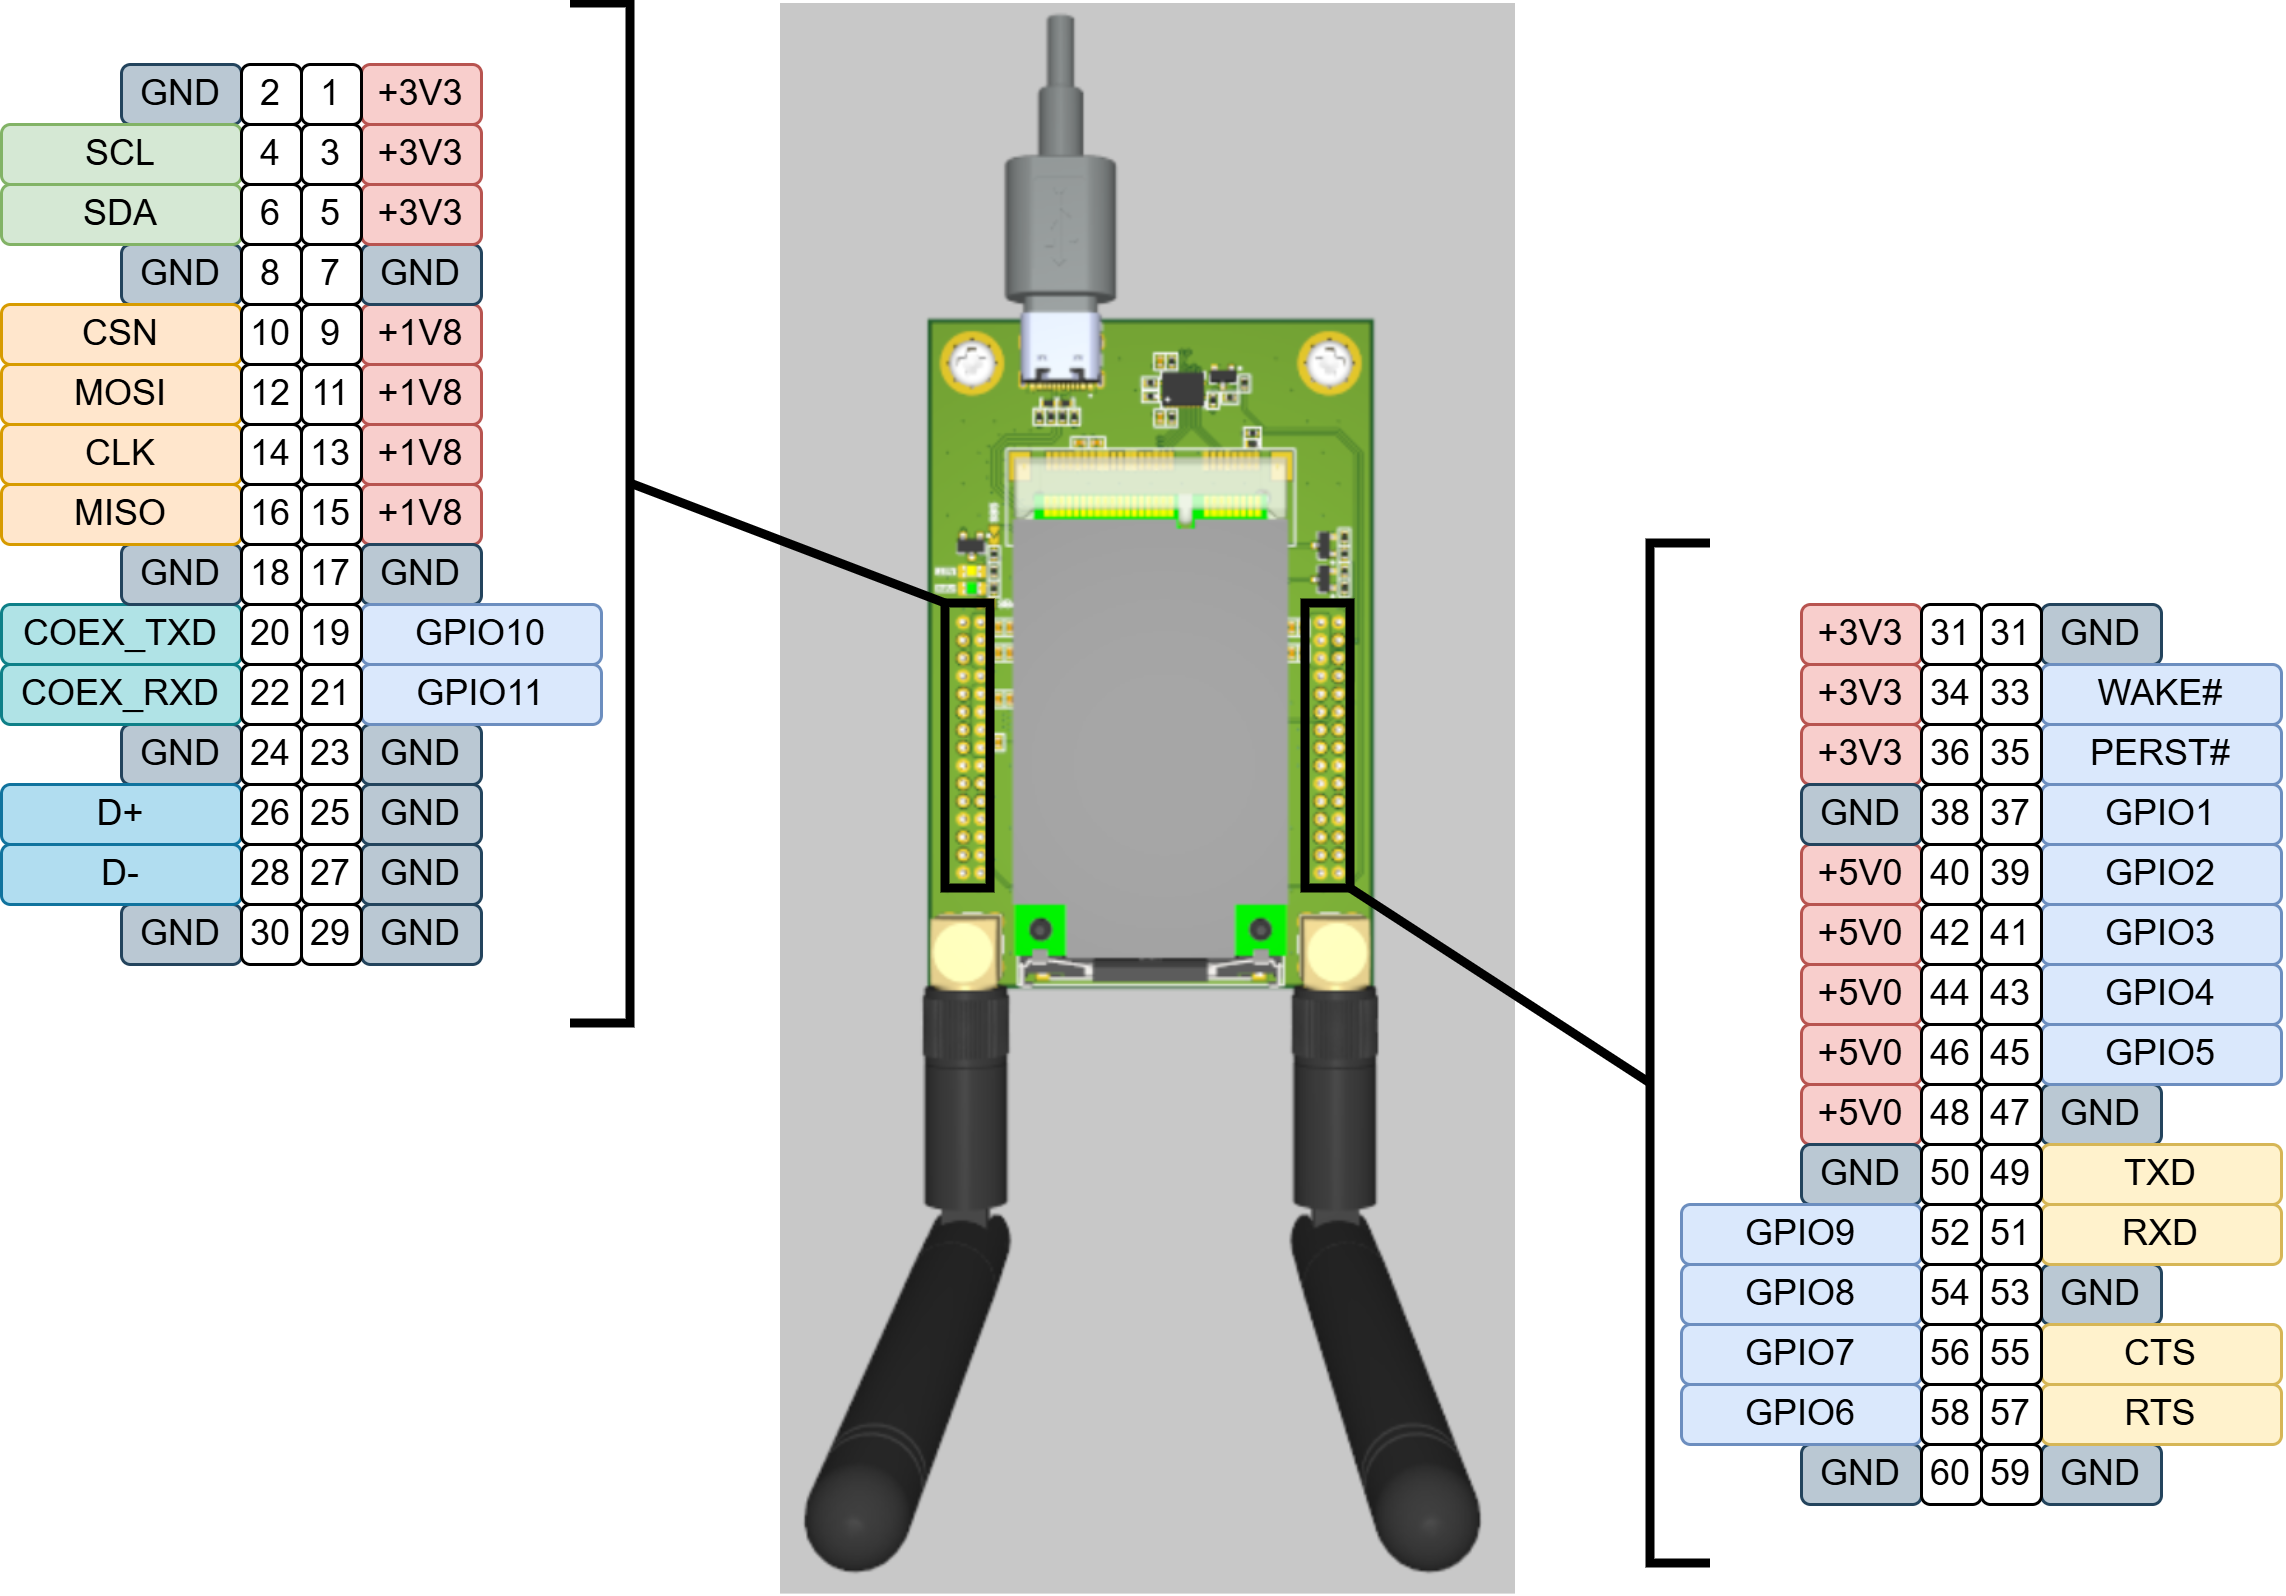
\includegraphics[width=0.8\textwidth]{figures/Adapter_Board_Definition.drawio.png}
                    \caption{Sơ đồ chân Module Adapter}
                \end{figure}

        \subsubsection{Xử lý dữ liệu}
            \dots\footnote{phần mềm}

    \newpage
    \subsection{Hardware}
        \subsubsection{Sơ đồ khối Phần cứng}
            \begin{figure}[h]
                \centering
                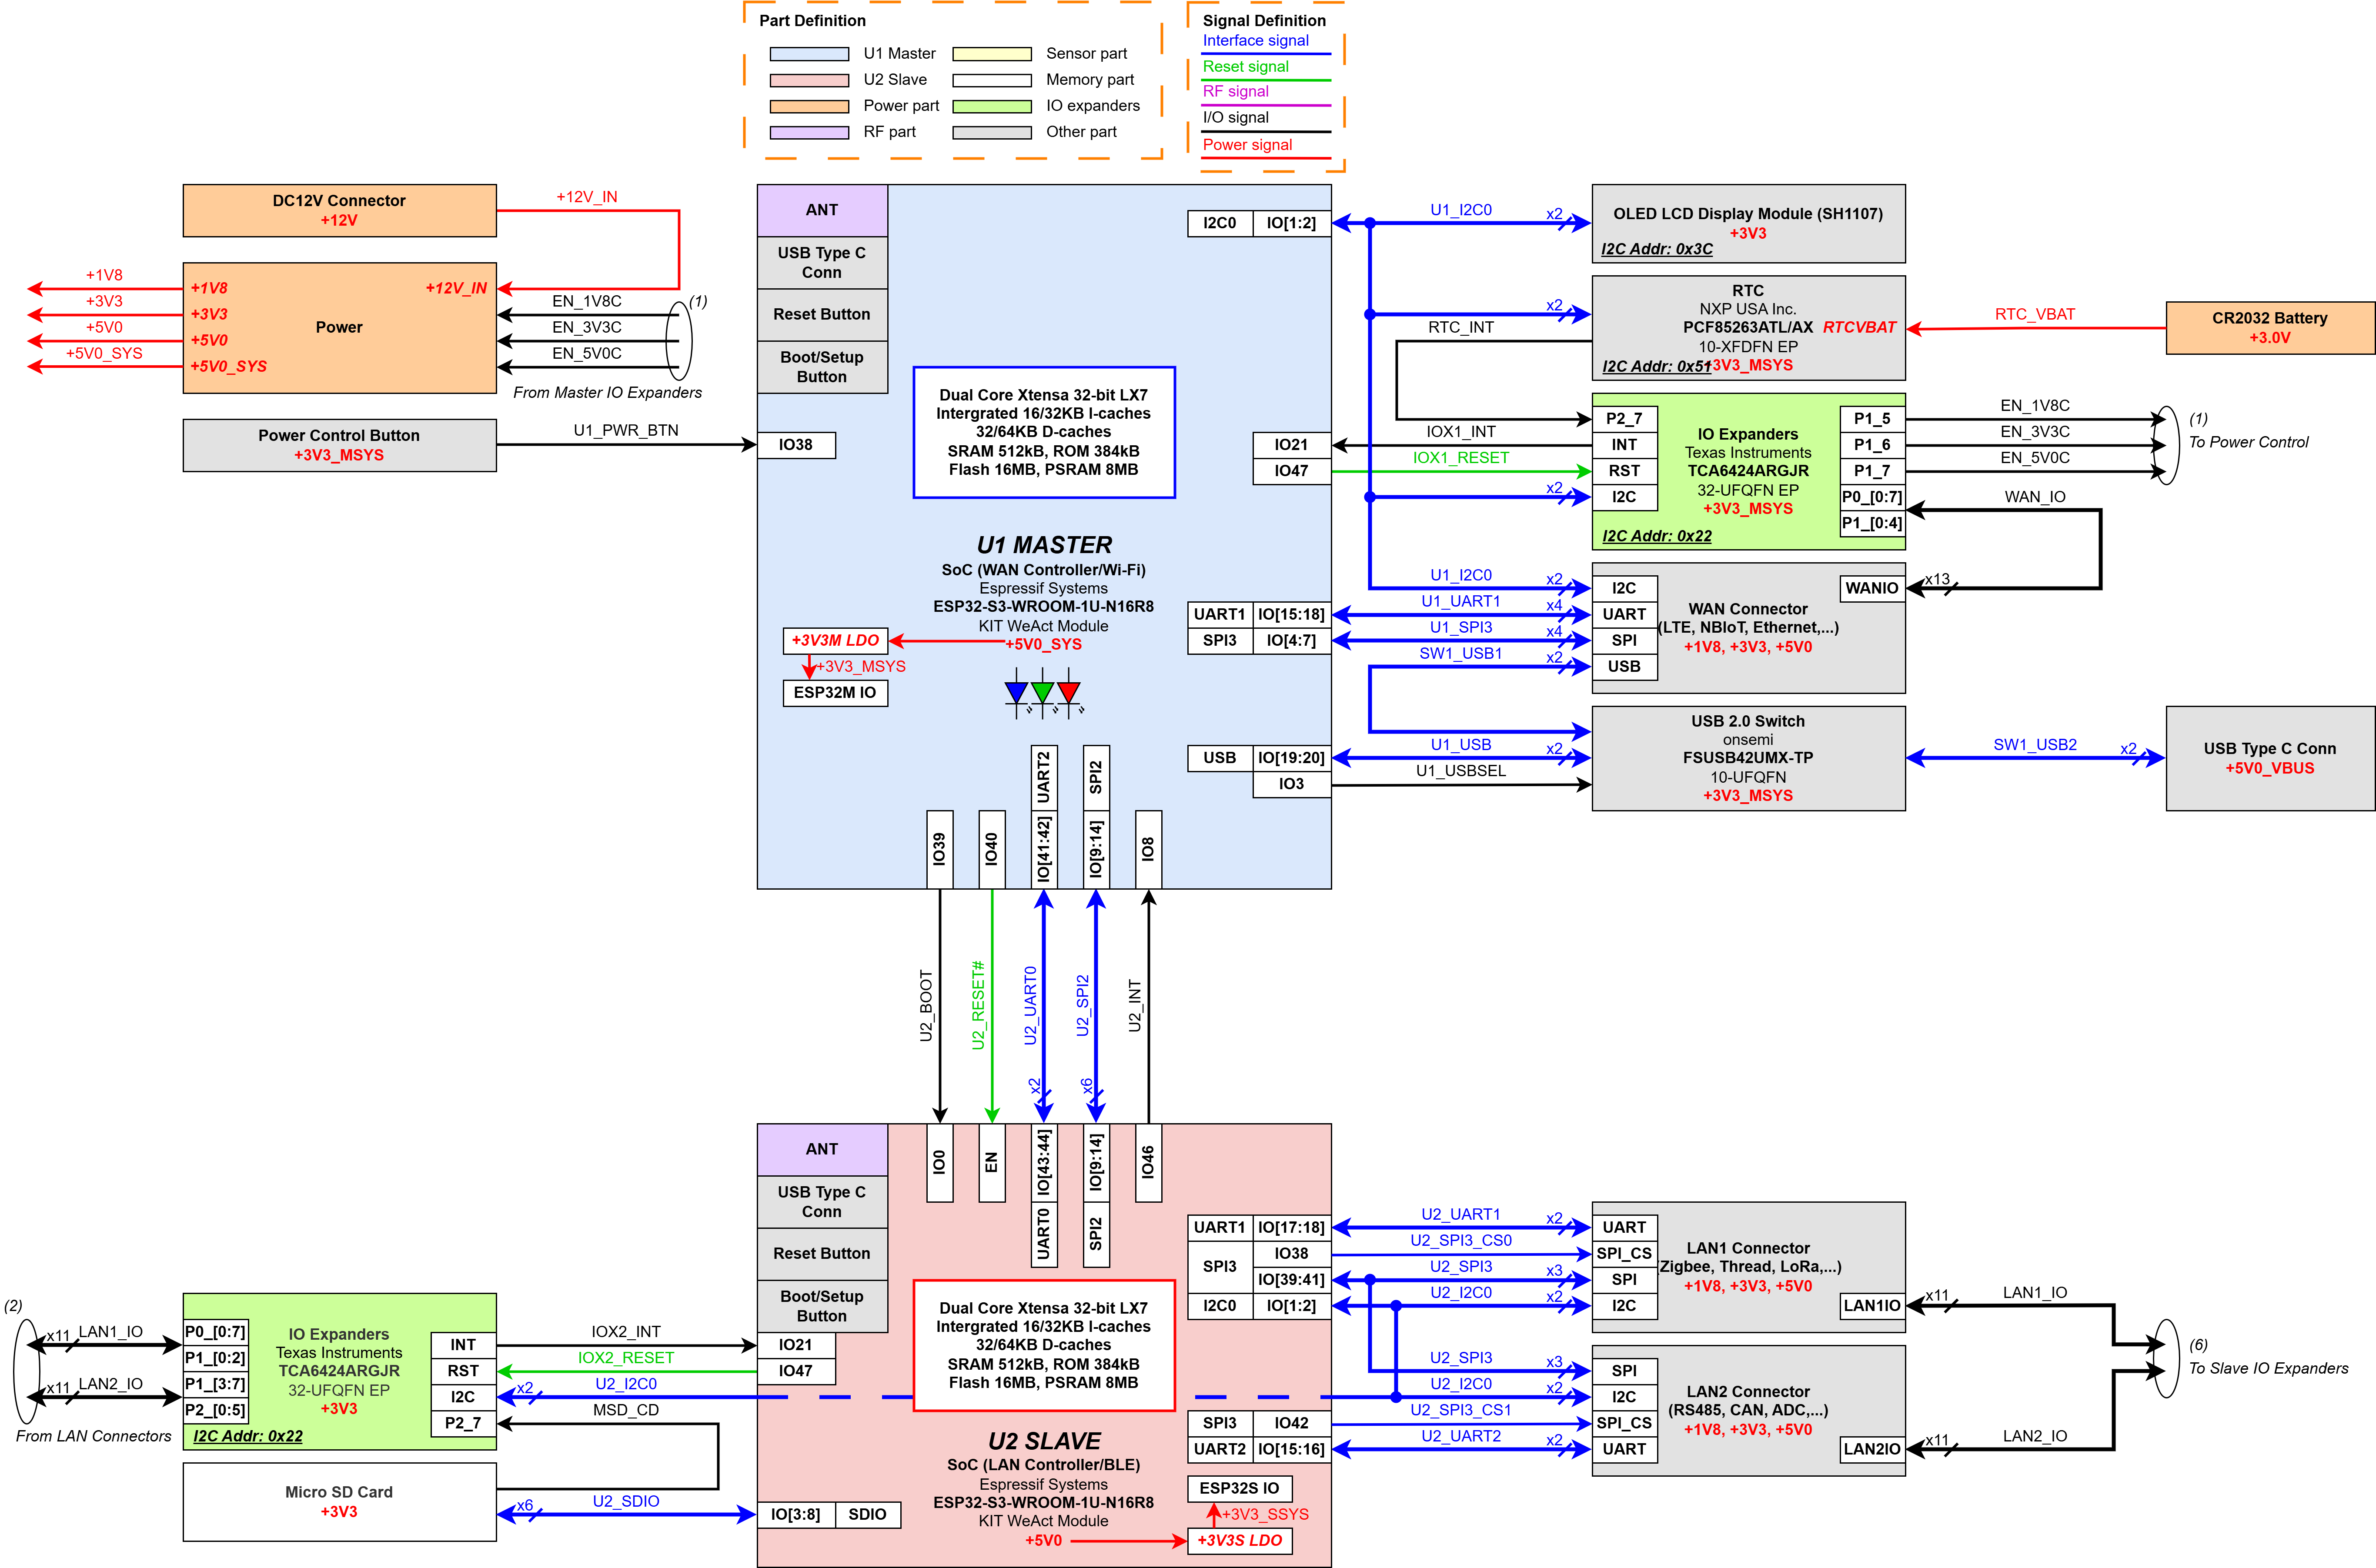
\includegraphics[width=\textwidth]{figures/BlockDiagram_Prototype_ModularIoTGateway-System Diagram.drawio.png}
                \caption{Sơ đồ khối Phần cứng}
            \end{figure}
            \dots

        \newpage
        \subsubsection{Hệ thống nguồn}
            \begin{figure}[h]
                \centering
                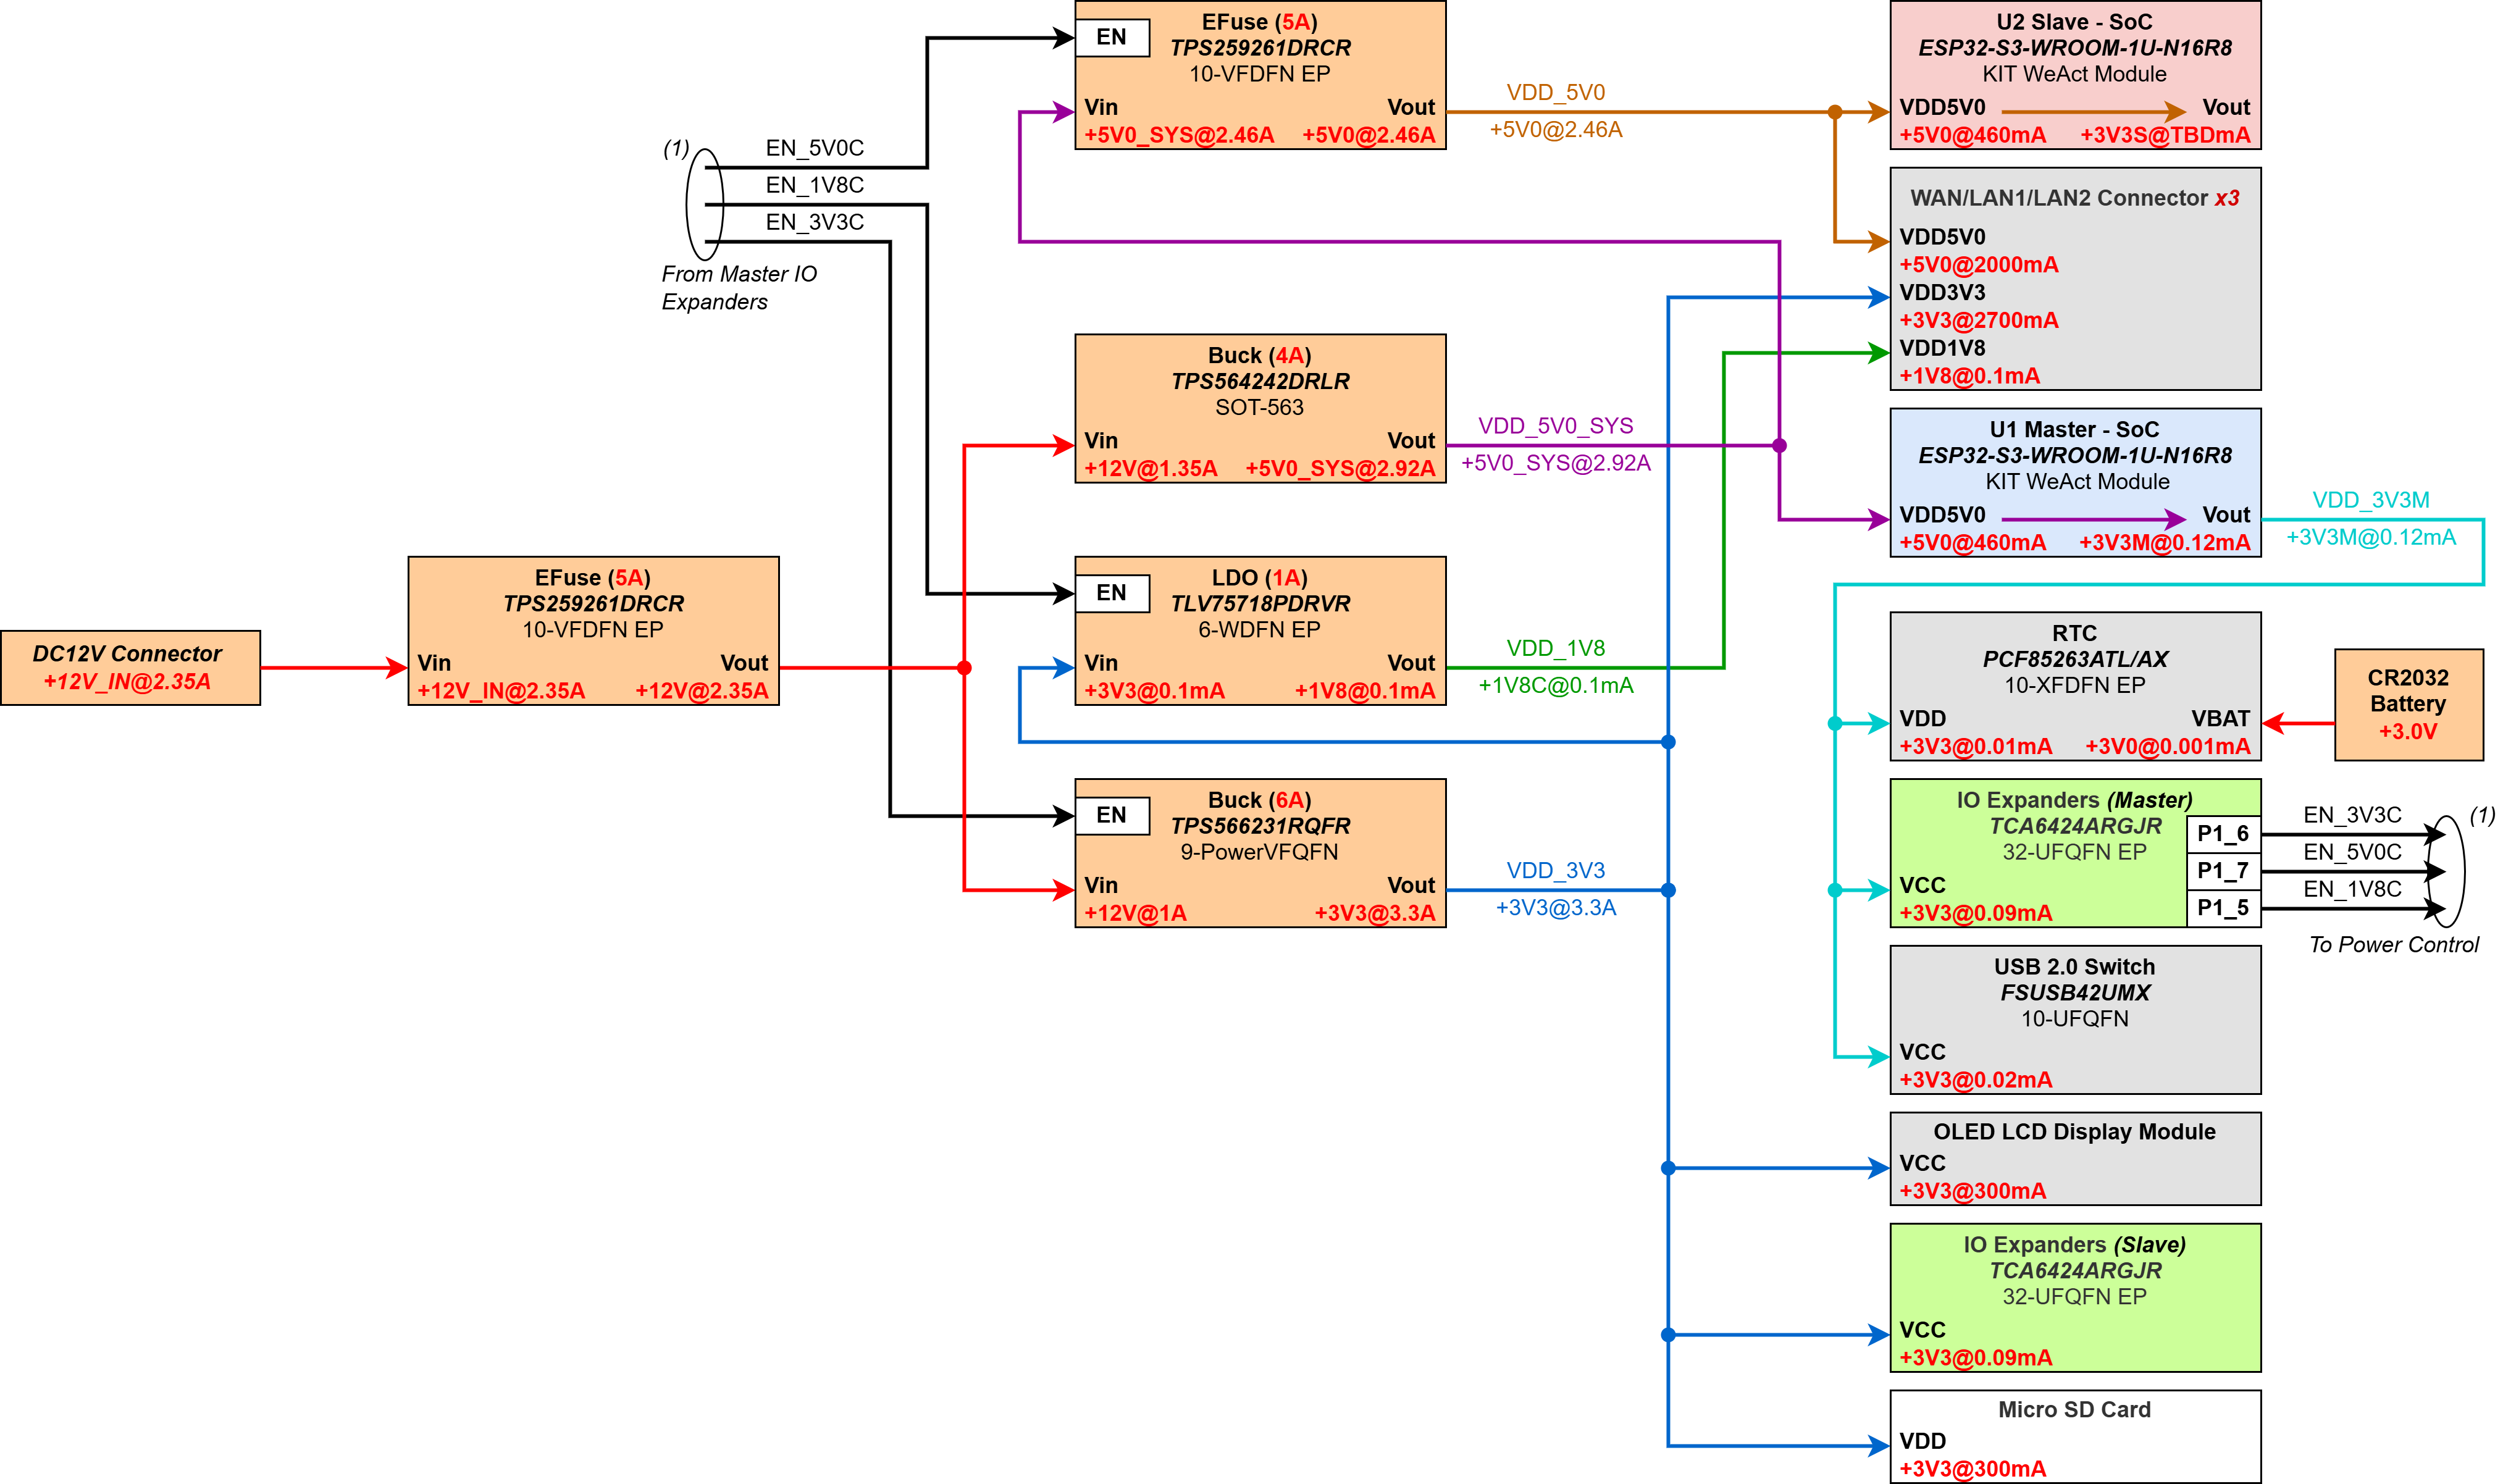
\includegraphics[width=\textwidth]{figures/BlockDiagram_Prototype_ModularIoTGateway-Power Diagram.drawio.png}
                \caption{Sơ đồ hệ thống nguồn}
            \end{figure}
            \dots

        \subsubsection{Thiết kế Mạch nguyên lý (Schematic)}
            \paragraph{Thiết kế Mạch xử lý trung tâm}
            \paragraph{Thiết kế Mạch nguồn}
            \paragraph{Thiết kế Mạch USB}
            \paragraph{Thiết kế Mạch IO Expander}
            \paragraph{Thiết kế Mạch RTC}
            \paragraph{Thiết kế Mạch Micro SD Card}
            \paragraph{Thiết kế Mạch Module Adapter}
        
        \subsubsection{Thiết kế PCB}
            \paragraph{Stack-up và Impedance control}
                \begin{enumerate}
                    \item \textbf{Stack-up:}
                    \begin{itemize}
                        \item Lựa chọn Stack-up: Thiết kế có nhiều kênh tín hiệu tốc độ cao, yêu cầu cần kiểm soát trở kháng và chống nhiễu, và yêu cầu nhiều rail nguồn khác nhau. Do đó, lựa chọn Stack-up 6 lớp nhằm đáp ứng các yêu cầu này với cấu trúc sau:
                        
                        \begin{longtable}{|l|l|l|}
                            \hline
                            \textbf{Layer} & \textbf{Ưu tiên} & \textbf{Mô tả} \\\hline
                            \endfirsthead
                            \hline
                            \textbf{Layer} & \textbf{Ưu tiên} & \textbf{Mô tả} \\\hline
                            \endhead
                            \hline
                            \endfoot
                            % \hline
                            \endlastfoot  
                            
                            \textbf{Layer 1} & High-speed Signal \& Power & Tín hiệu tốc độ cao và Nguồn \\\hline
                            \textbf{Layer 2} & Ground Plane & Lớp GND tham chiếu cho tín hiệu tốc độ cao ở Layer 1 \\\hline
                            \textbf{Layer 3} & Power Plane & Rail nguồn \\\hline
                            \textbf{Layer 4} & Low-speed Signal & Tín hiệu tốc độ thấp \\\hline
                            \textbf{Layer 5} & Ground Plane & Lớp GND tham chiếu cho tín hiệu tốc độ cao ở Layer 6 \\\hline
                            \textbf{Layer 6} & High-speed Signal \& Power & Tín hiệu tốc độ cao và Nguồn \\\hline
                        \end{longtable}
                        \item Trong thiết kế stack-up này vừa đảm bảo được có 2 layer cho tín hiệu tốc độ cao và 3 layer cho hệ thống nguồn, là vừa đủ để đảm bảo các yêu cầu về tính toàn vẹn tín hiệu và chống nhiễu, đồng thời vẫn giữ chi phí sản xuất PCB ở mức hợp lý. Ngoài ra, layer 3 (nguồn) và layer 2 (đất) đặt cạnh nhau tạo ra một tụ điện giúp ổn định hệ thống. Nguồn và tín hiệu tốc độ cao nằm cùng layer sẽ được layer tách biệt và được che phủ tránh ảnh hưởng bởi nhiễu chéo, đặc biệt là nguồn switching và tín hiệu tốc độ cao đều có tần số hoạt động rất lớn có thể gây nhiễu chéo.
                        \item Trong các thiết kế stack-up có các thiết kế tham khảo như sử dụng layer ở trong dùng cho tín hiệu tốc độ cao, ví dụ như thay thế Layer 4 để dùng cho High-speed Signal. Điều này giúp chống nhiễu tốt hơn, mang lại sự ổn định hơn do đồng nhất hơn khi nằm giữa cùng hai vật liệu cách điện giống nhau, thay vì tiếp xúc với không khí như ở layer ngoài cùng. Tuy nhiên, stack-up như vậy buộc layer 3 phải là Ground Plane, điều này làm giảm đi không gian để layer nguồn. Các tín hiệu tốc độ cao như SPI hay USB trong thiết kế cũng chưa đạt tới tần số cao đến mức cần phải bảo vệ nghiệm ngặt mặc dù cũng cần phải đảm bảo trở kháng và các kỹ thuật đảm bảo toàn vẹn tín hiệu. Và việc chỉ có một layer cho tín hiệu tốc độ cao thay vì hai cũng làm giảm đáng kể không gian layout không cần thiết.
                    \end{itemize}
                    \item \textbf{Impedance control:}
                    \begin{itemize}
                        \item Các tín hiệu tốc độ cao có yêu cầu về trở kháng nhằm đảm bảo tính toàn vẹn tín hiệu và giảm phát xạ EMI. Các tiêu chuẩn trở kháng được áp dụng trong thiết kế:
                        \begin{itemize}
                            \item Trở kháng cho tín hiệu Coplanar single-ended: $50\Omega\pm10\%$ cho tín hiệu SDIO, SPI, I2C.
                            \item Trở kháng cho tín hiệu Coplanar differential-pair: $90\Omega\pm10\%$ cho tín hiệu cặp vi sai USB.
                        \end{itemize}
                        \item Để đạt được trở kháng mục tiêu, các tín hiệu phải đi đúng kích thước và cấu trúc dựa trên tính toán từ các thông số vật liệu của stack-up. Dưới đây là bảng thông số và kích thước đường dây:
                        \begin{figure}[h]
                            \centering
                            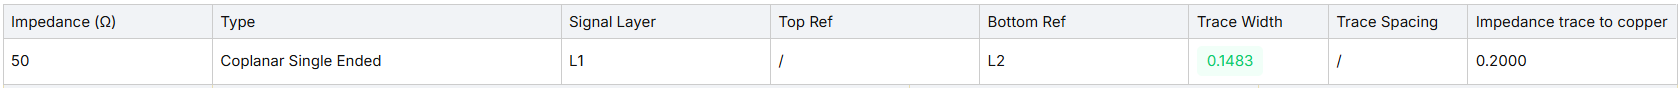
\includegraphics[width=\textwidth]{figures/impedance_50R.png}
                            \caption{Kích thước dây cho tín hiệu Coplanar single-ended $50\Omega\pm10\%$ (đơn vị: mm)}
                        \end{figure}
                        \begin{figure}[h]
                            \centering
                            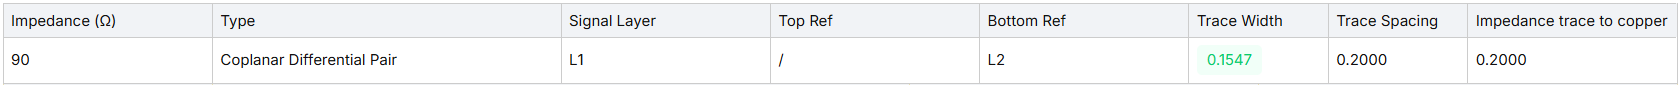
\includegraphics[width=\textwidth]{figures/impedance_90R.png}
                            \caption{Kích thước dây cho tín hiệu Coplanar differential-pair $90\Omega\pm10\%$ (đơn vị: mm)}
                        \end{figure}
                        \begin{figure}[h]
                            \centering
                            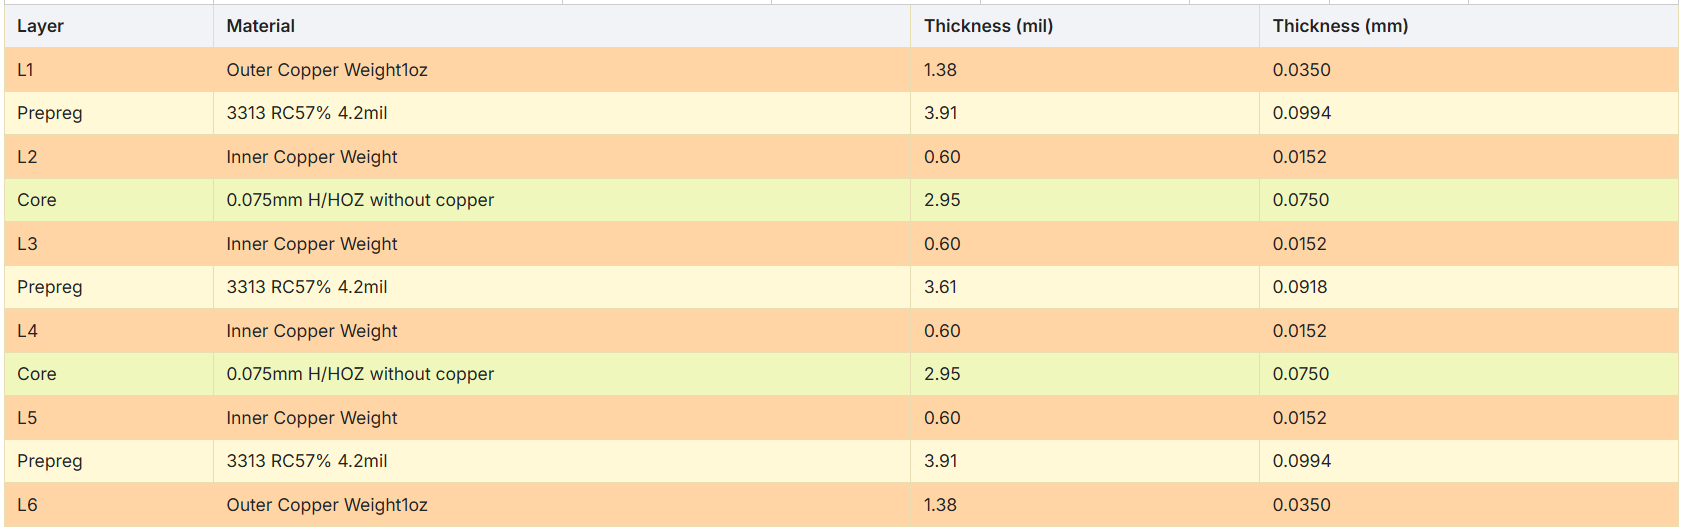
\includegraphics[width=\textwidth]{figures/jlcpcb_stackup.png}
                            \caption{Thông số stack-up theo tiêu chuẩn của đơn vị gia công JLCPCB}
                        \end{figure}
                            
                    \end{itemize}
                \end{enumerate}
                
            \paragraph{Quy hoạch, bố trí linh kiện (Component placement/Floor-planning):}
                Việc quy hoạch, bố trí linh kiện đảm bảo được những yếu tố:
                \begin{enumerate}
                    \item Phân vùng quy hoạch cho các chức năng như khu vực nguồn, khu vực xử lý trung tâm, khu vực ngoại vi, \dots
                    \item Quy hoạch các khối quan trọng như khối xử lý trung tâm ở vị trí dễ dàng kết nối với các khối khác.
                    \item Quy hoạch để các tín hiệu tốc độ cao ngắn nhất có thể.
                    \item Quy hoạch các thành phần dễ gây nhiễu ra xa các khu vực nhạy cảm, hay các thành phần cần được chống nhiễu xa khỏi các khu vực nhiễu mạnh.
                    \item Quy hoạch cho các khu vực RF ở góc hoặc rìa, đặt đủ xa và chéo góc để giảm hiện tương các sóng vô tuyến giao thoa với nhau.
                    \item Bố trí các linh kiện theo từng khối chức năng.
                    \item Bố trí các cổng kết nối hay những thành phần ảnh hưởng đến hình dạng board và kết cấu khung cơ khí.
                    \item \dots
                \end{enumerate}

            \paragraph{Kỹ thuật chống nhiễu}
                \begin{enumerate}
                    \item \textbf{Nguyên lý lồng Faraday:} Toàn bộ board được phủ GND xung quanh để chống lại nhiễu từ môi trường, các tín hiệu, linh kiện hoạt động ở tần số cao như tín hiệu tốc độ cao hay khối thạch anh cần được phủ ground và dùng via stitching xung quanh để tạo thành một lồng chắn sóng, tránh bị nhiễu và phát xạ ra các thành phần xung quanh.
                    \begin{figure}[h]
                        \centering
                        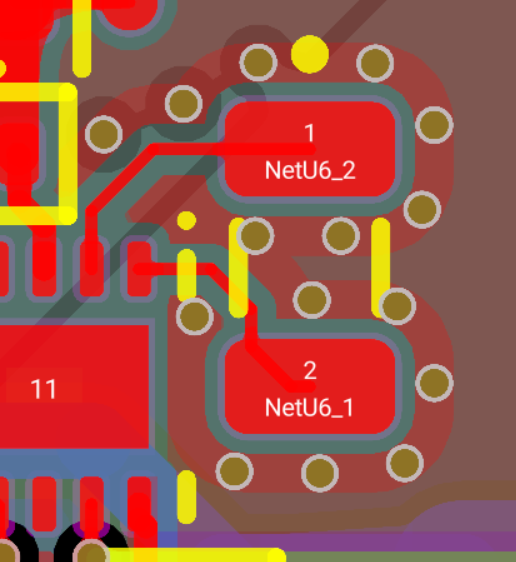
\includegraphics[height=0.45\textwidth]{figures/crysal_shielding_2D.png}
                        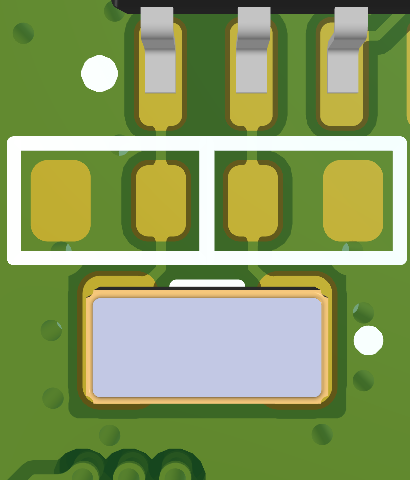
\includegraphics[height=0.45\textwidth]{figures/crysal_shielding_3D.png}
                        \caption{{Phủ GND Shielding và stitching via xung quanh thạch anh.}}
                    \end{figure}
                    \begin{figure}[h]
                        \centering
                        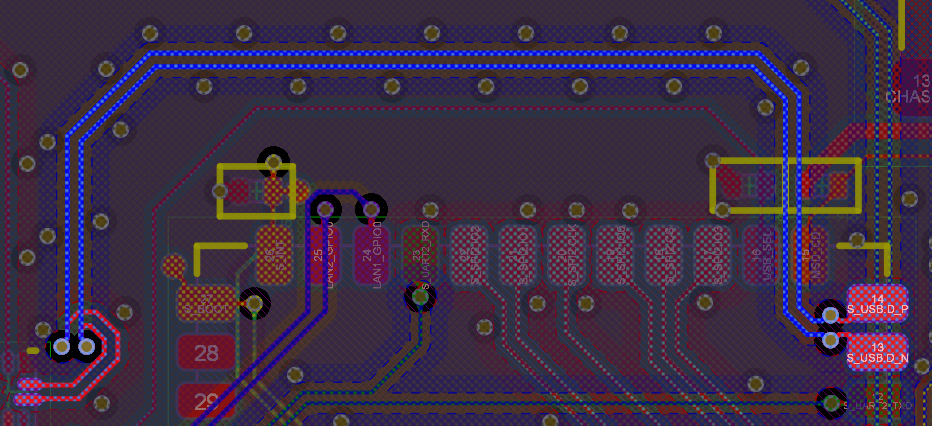
\includegraphics[width=0.8\textwidth]{figures/USB_shielding_2D.png}
                        \caption{{Phủ GND Shielding và stitching via xung quanh tín hiệu USB.}}
                    \end{figure}
                    \item Tránh tạo vòng lặp lớn, khi mà các tín hiệu đi qua các mặt phẳng đất không liên tục, việc này dẫn đến return path không trở về theo đường có trở kháng nhỏ nhất, tạo ra các vòng lặp lớn gây phát xạ nhiễu.
                \end{enumerate}

            \paragraph{Kỹ thuật layout Nguồn}
                \begin{enumerate}
                    \item \textbf{Tối ưu hóa current loop:} Các tụ đầu vào và đầu ra cần được đặt sát nhau nhất có thể và đặt gần cắc chân của IC nguồn hay cuộn cảm. Các linh kiện phải được bố trí sát nhau và giảm tối thiểu diện tích current loop nhằm giảm cảm kháng ký sinh và hạn chế bức xạ EMI.
                    \item \textbf{Xử lý điểm switching:} Tại các chân đầu ra của các IC nguồn switching là vị trí chuyển mạch tần số cao, vị trí này cần đường đi dây ngắn nhất và rộng có thể nhằm giảm bức xạ điện từ và đảm bảo khả năng chịu dòng xung lớn. Tuyệt đối không đi các đường tín hiệu nào ở gần hay ngay bên dưới vị trí chuyển mạch và cuộn cảm.
                    \item \textbf{Đường tín hiệu hồi tiếp:} Đường hồi tiếp nên đi tránh xa khỏi điểm switching, phủ GND xung quanh để tạo lớp chắn khỏi nhiễu từ nguồn, GND của đường hồi tiếp phải lấy từ chân GND của IC hoặc Analog GND, không sử dụng Power GND vì GND này đang chịu ảnh hưởng bởi mạch switching có thể làm nhiểu tín hiệu hồi tiếp. Điểm lấy điện áp cho tín hiệu hồi tiếp nên là điểm sau tụ điện đầu ra, là điểm khi nguồn điện đã ổn định
                    \item \textbf{Bố trí linh kiện:} Các linh kiện phụ trợ như điện trở, tụ điện cho các chức năng soft-start (khởi động mềm), bootstrap, giới hạn dòng cần được đặt sát chân tín hiệu của IC nguồn và sử dụng GND từ chân của IC nguồn hoặc Analog GND.
                    \item \textbf{Quản lý nhiệt:} Các lớp GND của nguồn nên được bố trí nhiều via ngay dưới pad tản nhiệt của IC và xung quanh các vùng GND xung quanh giúp tản nhiệt nhanh xuống các lớp phủ GND rộng lớn ở các layer bên dưới.
                    \item \textbf{Thiết kế mạng phân phối nguồn (Power Distribution Network - PDN):} Mục tiêu của thiết kế PDN là duy trì trở kháng thấp trên toàn dải tần số hoạt động, từ DC đến tần số chuyển mạch (Switching Frequency) và tần số xung nhịp của MCU.
                    \begin{itemize}
                        \item Các lớp nguồn và đất được bố trí xen kẻ nhau: Layer 1 (Power) - Layer 2 (Ground) - Layer 3 (Power) tạo ra các tụ điện phẳng ký sinh giúp lọc nhiễu và đảm bảo độ ổn định nguồn.
                        \item Các đường dẫn dòng được layout dạng mặt phẳng hoặc đường mạch rất rộng nhằm giảm điện trở thuần, hạn chế sụt áp và giảm cảm kháng ký sinh.
                        \item Tụ điện được thiết kế thành dải các tụ có giá trị từ nhỏ đến lớn, gồm các tụ rất nhỏ (18pF) đặt sát ngay chân nguồn IC để triệt tiêu nhiễu cao tần, và các tụ điện lớn cho hoạt động chuyển mạch của nguồn và ổn định điện áp.
                        \item Dây dẫn nguồn được định tuyến thành những mảng đồng lớn tăng khả năng tải dòng lớn, giảm trở kháng trên đường nguồn gây sụt áp trên đường nguồn, tăng khả năng tản nhiệt và giảm khả năng phát sinh nhiệt do năng lượng bị tiêu hao do trở kháng cao.
                        \item Khi đường nguồn định tuyển càng nhỏ sẽ làm tăng cảm kháng ký sinh, khi có các xung điện như gần nguồn xung, thiết bị thay đổi tải tức thời hay hoạt động với tần số cao, các đường nguồn nhỏ trở thành cuộn cảm trên suốt đường dây, điều này gây phát sinh nhiễu điện từ và hiện tượng Ringing làm cho điện áp dao động không ổn định.
                    \end{itemize}
                \end{enumerate}

            \paragraph{Kỹ thuật layout tín hiệu tốc độ cao}
                \begin{enumerate}
                    \item \textbf{Định tuyến cặp vi sai:}
                    \begin{itemize}
                        \item Cặp tín hiệu vi sai USB yêu cầu đặt trở kháng mục tiêu là $90\Omega\pm10\%$.
                        \item Định tuyến theo dạng Coplanar Differential-pair.
                        \item Đảm bảo chiều dài của mỗi dây trong cặp vi sai luôn bằng nhau và phải được định tuyến song song và đối xứng trong suốt chiều dài đường truyền.
                    \end{itemize}
                    \item \textbf{Định tuyến song song:}
                    \begin{itemize}
                        \item Tất cả các đường tín hiệu trong bus SPI và SDIO phải luôn đảm bảo đặt trở kháng mục tiêu là $50\Omega\pm10\%$.
                        \item Các đường tín hiệu được định tuyến theo dạng Coplanar Single-ended. Riêng với đường tín hiệu clock phải luôn được phủ GND suốt cả đường truyền.
                        \item Đảm bảo chiều dài của tất cả các đường truyền là bằng nhau bằng các kỹ thuật length matching.
                    \end{itemize}
                    \item \textbf{Kiểm soát nhiễu:}
                    \begin{itemize}
                        \item Hạn chế tối đa việc chuyển lớp trên các tín hiệu tốc độ cao.
                        \item Tránh định tuyến các tín hiệu khác song song với các đường tín hiệu tốc độ cao, nếu bắt buộc thì phải đi vuông góc và tiếp xúc ít nhất có thể.
                        \item Lớp GND tham chiếu phải liền mạch, không để các tín hiệu tốc độ cao đi qua những phần GND bị gián đoạn.
                        \item Tín hiệu tốc độ cao cần phải được che chắn và hạn chế định tuyến gần những vùng nhiễu mạnh như bộ dao động thạch anh, nguồn xung, cuộn cảm, \dots
                    \end{itemize}
                \end{enumerate}

        
        \subsubsection{Phân tích và Mô phỏng}
            \paragraph{Impedance Control}
            \paragraph{Power Distribution Network - PDN}
                \begin{enumerate}
                    \item \textbf{Mạng nguồn:}
                    \item \textbf{Phân tích Sụt áp trên đường dây:}
                    \item \textbf{Phân tích Mật độ dòng điện:}
                    \begin{itemize}
                        \item Mật độ dòng điện là đại lượng thể hiện mức độ tập trung dòng điện qua một đơn vị tiết diện. Khi mật độ dòng điện quá cao, các electron sẽ va chạm nhiều hơn với mạng tinh thể đồng, sinh ra nhiều nhiệt. Lượng nhiệt này, nếu đủ lớn, sẽ làm nóng chảy mạch hoặc gây sụt áp.
                        \item Theo tiêu chuẩn IPC-2221, đường mạch phải đủ rộng để tăng nhiệt độ không quá $10\,^\circ\mathrm{C}$.
                    \end{itemize}
                \end{enumerate}
    \subsection{Firmware và Software}
        \dots\footnote{phần mềm}